\documentclass[12pt,a4paper]{book}
%宏包
\usepackage{amsmath}
\usepackage{amssymb}
\usepackage{amsthm}
\usepackage{mathrsfs}
\usepackage{geometry}
\usepackage{natbib}%bibtex
\usepackage[dvipsnames]{xcolor}
\usepackage{tcolorbox}
\usepackage{enumerate}
\usepackage{tikz}
\usepackage{tikz-cd}
\usepackage{quiver}
\usepackage{float}
\usepackage{caption}
\usepackage[colorlinks,linkcolor=blue]{hyperref}
\usepackage{enumerate}
\usepackage{tabularx}%控制列宽
\usepackage{xr}%跨文件引用
\externaldocument{D:/latex/book/algebra/algebra}
%页面设置
\linespread{1.2}
\geometry{a4paper,left=2cm,right=2cm,top=2.5cm,bottom=2cm}
%\geometry{a4paper,left=2cm,right=2cm,top=2.5cm,bottom=2cm}

%环境和宏指令
\newenvironment{prooff}{{\noindent\it\textcolor{cyan!40!black}{Proof}:}\,}{\par}
\newenvironment{proofff}{{\noindent\it\textcolor{cyan!40!black}{Proof of the lemma}:}\,}{\qed \par}
\newcommand{\bbrace}[1]{\left\{ #1 \right\} }
\newcommand{\bb}[1]{\mathbb{#1}}
\newcommand{\p}{^{\prime}}
\renewcommand{\mod}[1]{(\text{mod}\,#1)}
\newcommand{\blue}[1]{\textcolor{blue}{#1}}
\newcommand{\spec}[1]{\text{Spec}({#1})}
\newcommand{\rarr}[1]{\xrightarrow{#1}}
\newcommand{\larr}[1]{\xleftarrow{#1}}
\newcommand{\emptyy}{\underline{\quad}}
\newenvironment{enu}{\begin{enumerate}[(1)]}{\end{enumerate}}
%ctrl+点击文本返回代码  选中代码 ctrl+alt+j 为代码查找文本




%定理环境
\theoremstyle{definition}
\newtheorem{defn}{Definition}[section]
\newtheorem{coro}[defn]{Corollary}
\newtheorem{theo}[defn]{Theorem}
\newtheorem{exer}[defn]{Exercise}
\newtheorem{rema}[defn]{Remark}
\newtheorem{lem}[defn]{Lemma}
\newtheorem{prop}[defn]{Proposition}
\newtheorem{nota}[defn]{Notation}
\newtheorem{exam}[defn]{Example}


\title{2024-10-b} 
\begin{document}
\maketitle 
1. 1. In a long line of people arranged left to right, the 1013th person from the left is also the 1010th person from the right. How many people are in the line?
(A) 2021
(B) 2022
(C) 2023
(D) 2024
(E) 2025

2. What is $10!-7!\cdot 6$ !?
(A) -120
(B) 0
(C) 120
(D) 600
(E) 720

3. For how many integer values of $x$ is $|2 x| \leq 7 \pi$ ?
(A) 16
(B) 17
(C) 19
(D) 20
(E) 21

4. Balls numbered $1,2,3, \ldots$ are deposited in 5 bins, labeled $\mathrm{A}, \mathrm{B}, \mathrm{C}, \mathrm{D}$, and E , using the following procedure. Ball 1 is deposited in bin $A$, and balls 2 and 3 are deposited in bin $B$. The next 3 balls are deposited in bin C, the next 4 in bin D, and so on, cycling back to bin A after balls are deposited in bin E. (For example, balls numbered 22, 23, .., 28 are deposited in bin B at step 7 of this process.) In which bin is ball 2024 deposited?
(A) A
(B) B
(C) C
(D) D
(E) E

5. In the following expression, Melanie changed some of the plus signs to minus signs:

$$
1+3+5+7+\cdots+97+99
$$


When the new expression was evaluated, it was negative. What is the least number of plus signs that Melanie could have changed to minus signs?
(A) 14
(B) 15
(C) 16
(D) 17
(E) 18

6. A rectangle has integer length sides and an area of 2024. What is the least possible perimeter of the rectangle?
(A) 160
(B) 180
(C) 222
(D) 228
(E) 390

7. What is the remainder when $7^{2024}+7^{2025}+7^{2026}$ is divided by 19 ?
(A) 0
(B) 1
(C) 7
(D) 11
(E) 18

8. Let $N$ be the product of all the positive integer divisors of 42 . What is the units digit of $N$ ?
(A) 0
(B) 2
(C) 4
(D) 6
(E) 8

9. Real numbers $a, b$, and $c$ have arithmetic mean 0 . The arithmetic mean of $a^2, b^2$, and $c^2$ is 10 . What is the arithmetic mean of $a b, a c$, and $b c$ ?
(A) -5
(B) $-\frac{10}{3}$
(C) $-\frac{10}{9}$
(D) 0
(E) $\frac{10}{9}$

\begin{figure}[H]
    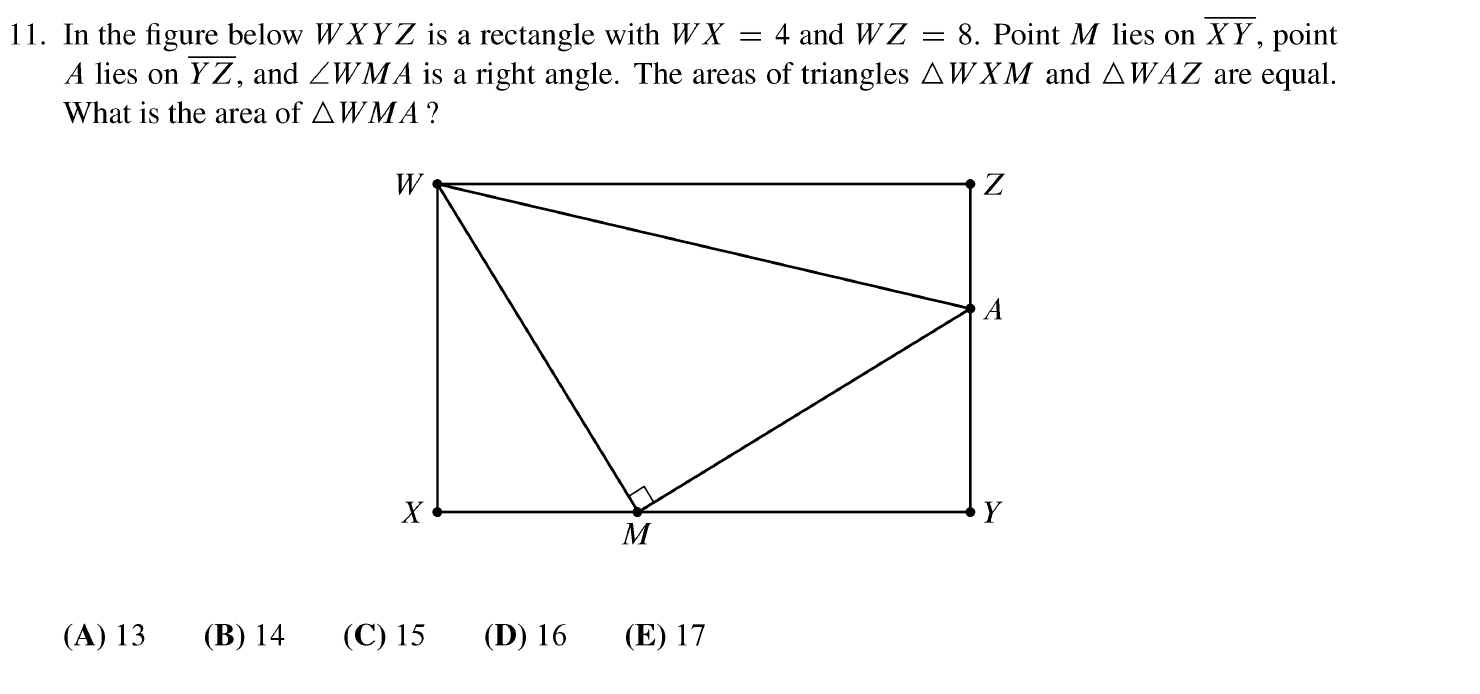
\includegraphics[height=0.3\textheight]{11.png}
\end{figure}
12. A group of 100 students from different countries meet at a mathematics competition. Each student speaks the same number of languages, and, for every pair of students A and B , student A speaks some language that student B does not speak, and student B speaks some language that student A does not speak. What is the least possible total number of languages spoken by all the students?
(A) 9
(B) 10
(C) 12
(D) 51
(E) 100

13. Positive integers $x$ and $y$ satisfy the equation $\sqrt{x}+\sqrt{y}=\sqrt{1183}$. What is the minimum possible value of $x+y$ ?
(A) 585
(B) 595
(C) 623
(D) 700
(E) 791

14. A dartboard is the region $B$ in the coordinate plane consisting of points $(x, y)$ such that $|x|+|y| \leq 8$. A target $T$ is the region where $\left(x^2+y^2-25\right)^2 \leq 49$. A dart is thrown and lands at a random point in $B$. The probability that the dart lands in $T$ can be expressed as $\frac{m}{n} \cdot \pi$, where $m$ and $n$ are relatively prime positive integers. What is $m+n$ ?
(A) 39
(B) 71
(C) 73
(D) 75
(E) 135

15. A list of 9 real numbers consists of $1,2.2,3.2,5.2,6.2$, and 7 , as well as $x, y$, and $z$ with $x \leq y \leq z$. The range of the list is 7 , and the mean and the median are both positive integers. How many ordered triples $(x, y, z)$ are possible?
(A) 1
(B) 2
(C) 3
(D) 4
(E) infinitely many

16. Jerry likes to play with numbers. One day, he wrote all the integers from 1 to 2024 on the whiteboard. Then he repeatedly chose four numbers on the whiteboard, erased them, and replaced them by either their sum or their product. (For example, Jerry's first step might have been to erase 1, 2, 3, and 5, and then write either 11, their sum, or 30, their product, on the whiteboard.) After repeatedly performing this operation, Jerry noticed that all the remaining numbers on the whiteboard were odd. What is the maximum possible number of integers on the whiteboard at that time?
(A) 1010
(B) 1011
(C) 1012
(D) 1013
(E) 1014

17. In a race among 5 snails, there is at most one tie, but that tie can involve any number of snails. For example, the result of the race might be that Dazzler is first; Abby, Cyrus, and Elroy are tied for second; and Bruna is fifth. How many different results of the race are possible?
(A) 180
(B) 361
(C) 420
(D) 431
(E) 720

18. How many different remainders can result when the 100 th power of an integer is divided by 125 ?
(A) 1
(B) 2
(C) 5
(D) 25
(E) 125
\begin{figure}[H]
    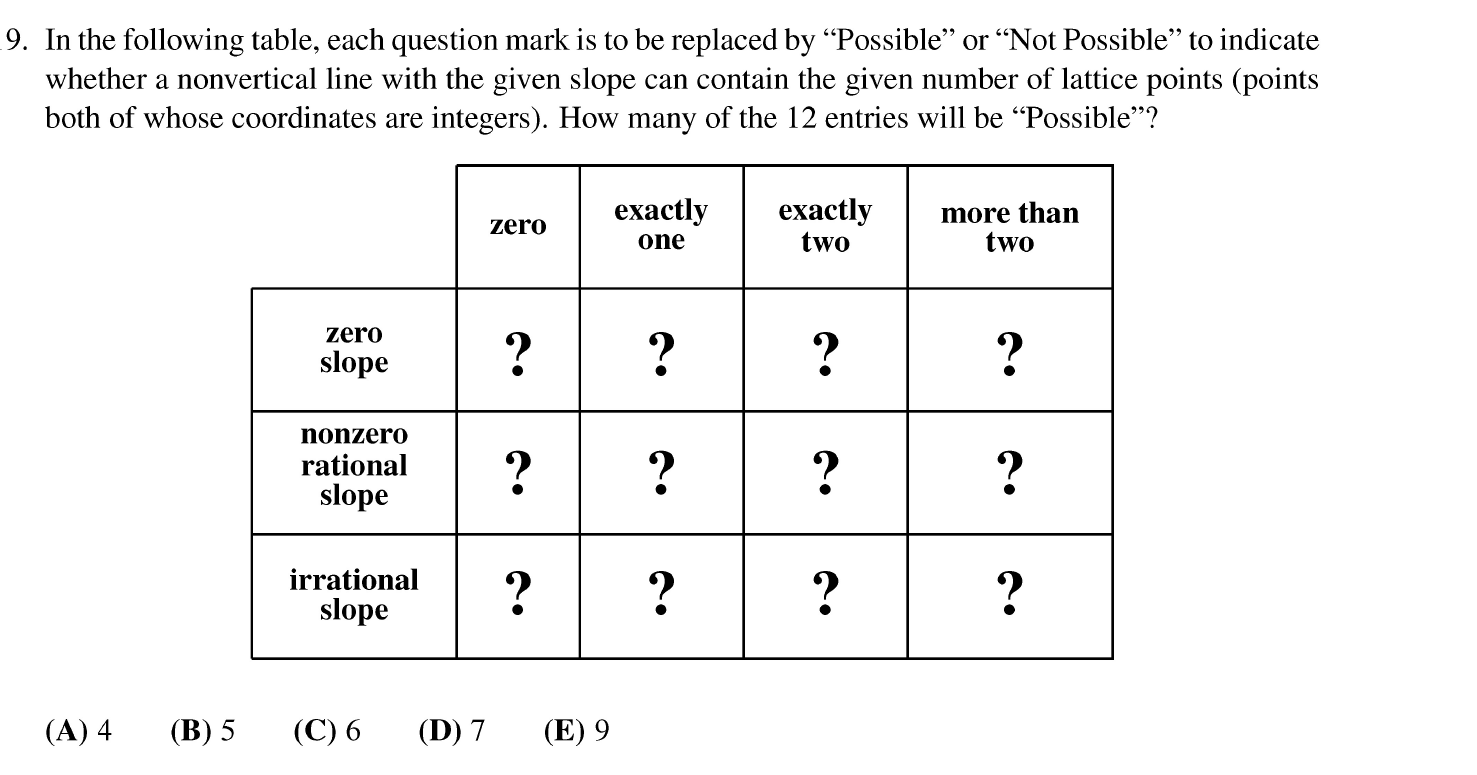
\includegraphics[height=0.3\textheight]{19.png}
\end{figure}
20. Three different pairs of shoes are placed in a row so that no left shoe is next to a right shoe from a different pair. In how many ways can these six shoes be lined up?
(A) 60
(B) 72
(C) 90
(D) 108
(E) 120
\begin{figure}[H]
    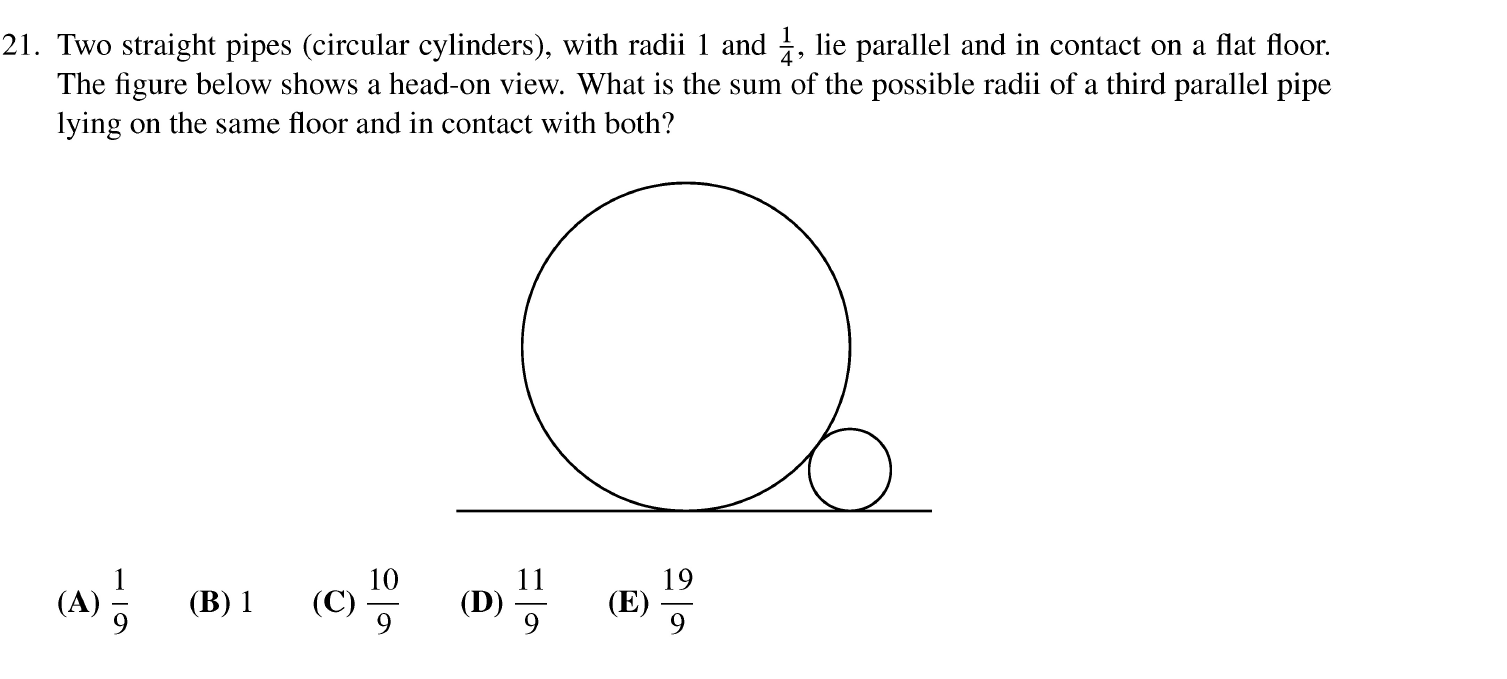
\includegraphics[height=0.3\textheight]{21.png}
\end{figure}

22. A group of 16 people will be partitioned into 4 indistinguishable 4-person committees. Each committee will have one chairperson and one secretary. The number of different ways to make these assignments can be written as $3^r M$, where $r$ and $M$ are positive integers and $M$ is not divisible by 3 . What is $r$ ?
(A) 5
(B) 6
(C) 7
(D) 8
(E) 9

23. The Fibonacci numbers are defined by $F_1=1, F_2=1$, and $F_n=F_{n-1}+F_{n-2}$ for $n \geq 3$. What is

$$
\frac{F_2}{F_1}+\frac{F_4}{F_2}+\frac{F_6}{F_3}+\cdots+\frac{F_{20}}{F_{10}} ?
$$

(A) 318
(B) 319
(C) 320
(D) 321
(E) 322

24. Let

$$
P(m)=\frac{m}{2}+\frac{m^2}{4}+\frac{m^4}{8}+\frac{m^8}{8} .
$$


How many of the values $P(2022), P(2023), P(2024)$, and $P(2025)$ are integers?
(A) 0
(B) 1
(C) 2
(D) 3
(E) 4

25
Each of 27 bricks (right rectangular prisms) has dimensions $a \times b \times c$, where $a, b$, and $c$ are pairwise relatively prime positive integers. These bricks are arranged to form a $3 \times 3 \times 3$ block, as shown on the left below. A 28th brick with the same dimensions is introduced, and these bricks are reconfigured into a $2 \times 2 \times 7$ block, shown on the right. The new block is 1 unit taller, 1 unit wider, and 1 unit deeper than the old one. What is $a+b+c$ ?
(A) 88
(B) 89
(C) 90
(D) 91
(E) 92

\begin{figure}[H]
    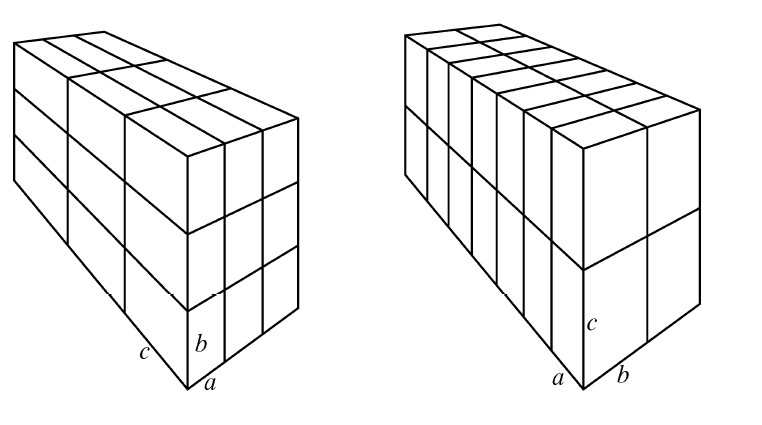
\includegraphics[height=0.3\textheight]{25-picture.png}
\end{figure}


\end{document}